\lecture{8}{19. Februar 2025}{Dislocations and strengthening mechanisms}

\section{Slipping}
Plastic deformation occurs by motion of dislocations in a process known as \textit{slip}. An applied shear stress can e.g. cause an edge dislocation (half plane of atoms) to move as shown in \textbf{\autoref{fig:f8_1}}.
\begin{figure} [ht]
  \centering
  \caption{Motion of an edge dislocation due to shear stress}
  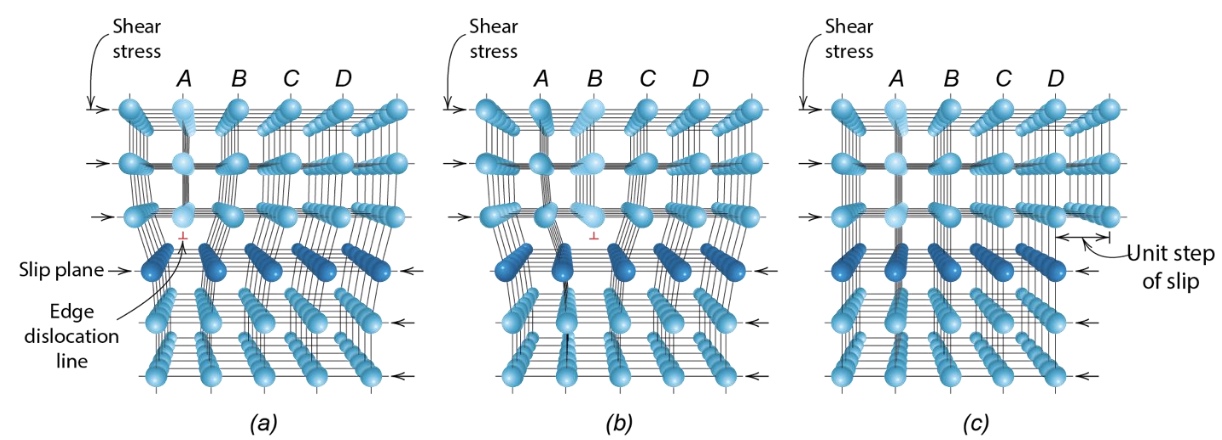
\includegraphics[width=0.5\linewidth]{./figures/f8_1.png}
  \label{fig:f8_1}
\end{figure}
During this process, atomic bonds are broken and reformed along the slip plane as the dislocation moves.


\subsection{Slip systems}
A \textit{slip system} is a combination of a \textit{slip plane} and a \textit{slip direction}. A slip plane is a crystallographic plane on which slip occurs most easily -- this is the plane with the highest planar density. A slip direction is the crystallographic direction along which slips occur most easily -- this is the direction with the highest linear density. 

For the FCC crystal structure the slip system is $\{111\} \left\langle 110 \right\rangle $. This means the dislocation motion is on the $\{111\}$ plane and in the $\left\langle 110 \right\rangle$ direction. This family of slip systems contains 12 ``different'' independent slip systems for FCC. The slip system for FCC is shown in \textbf{\autoref{fig:f8_2}}. For BCC and HCP other slip systems exist.

\begin{figure} [ht]
  \centering
  \caption{Slip system for FCC}
  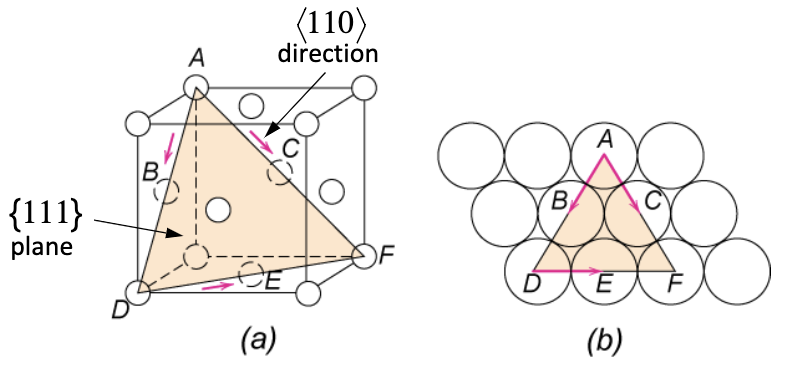
\includegraphics[width=0.5\linewidth]{./figures/f8_2.png}
  \label{fig:f8_2}
\end{figure}

\subsection{Slipping in single crystals}
When looking at a single crystal we do not have any grain boundaries. The slipping will happen along the slip planes, which can lead to ``stepping'', as a large number of dislocations will move along the same line. This is shown in \textbf{\autoref{fig:f8_3}}

\begin{figure} [ht]
  \centering
  \caption{Slipping in a single crystal}
  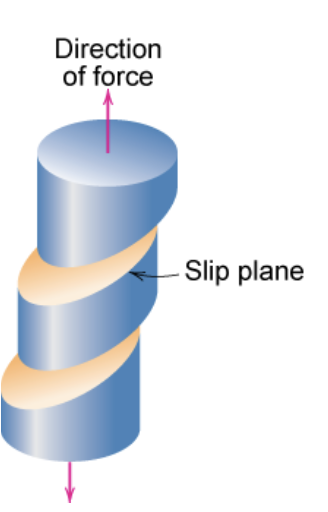
\includegraphics[width=0.25\linewidth]{./figures/f8_3.png}
  \label{fig:f8_3}
\end{figure}

\subsection{Slipping in polycrystalline materials}
Polycrystalline materials have many grains and with (often) random crystallopgraphic orientation of the grains. The slipping will therefore also happen pretty ``randomly'' on a microscopic scale, as the system will always slip in the most favourable direction. However, looking at the material macroscopically, one is able to draw some general conclusions. In general, individual grains will become distorted in a manner similar to the gross plastic deformation. On \textbf{\autoref{fig:f8_4}} a picture of the grains in a metal is shown before and after rolling -- it is easy to see that the grains have become distorted and have expanded in the horizontal direction. After this process, the material will often become somewhat anisotropic as the grains no longer are ``equal'' in all directions.

\begin{figure} [ht]
  \centering
  \caption{Distortion of grains due to slipping}
  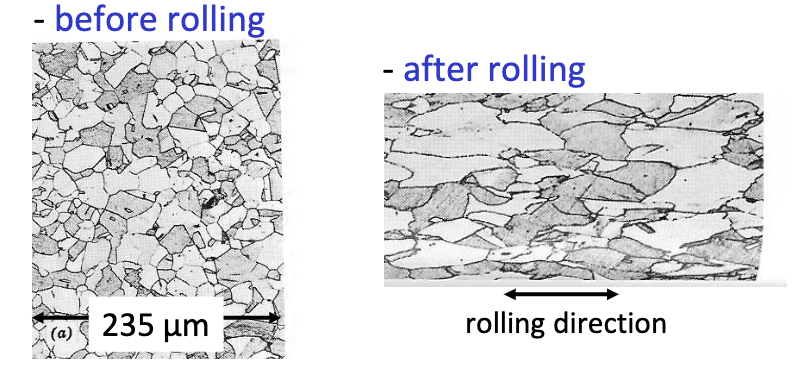
\includegraphics[width=0.6\linewidth]{./figures/f8_4.png}
  \label{fig:f8_4}
\end{figure}

\section{Strengthening mechanisms in metals}
For a metal to plastically deform dislocations must move. The quantities of strength and hardness are related to the mobility of dislocations -- if one decreases the dislocation mobility the metal will become stronger/harder and vice versa. All mechanisms for strengthening/hardening metals work by decreasing the mobility of dislocations. In this course we will focus on the following three methods of hardening.

\begin{itemize}
  \item Grain size reduction
  \item Solid solution strengthening
  \item Strain hardening (cold working)
\end{itemize}

\subsection{Grain size reduction}
Grain boundaries act as barriers of dislocation motion. This is because right at the boundary the slip plane changes direction (see \textbf{\autoref{fig:f8_5}}) which makes the slip plane discontinuous and therefore slipping will be inhibited. By reducing the grain size the total area of the grain boundaries will increase which provides more barriers to slipping and thus increasing the hardness and strength of the material. 

\begin{figure} [ht]
  \centering
  \caption{Slip planes across grain boundaries}
  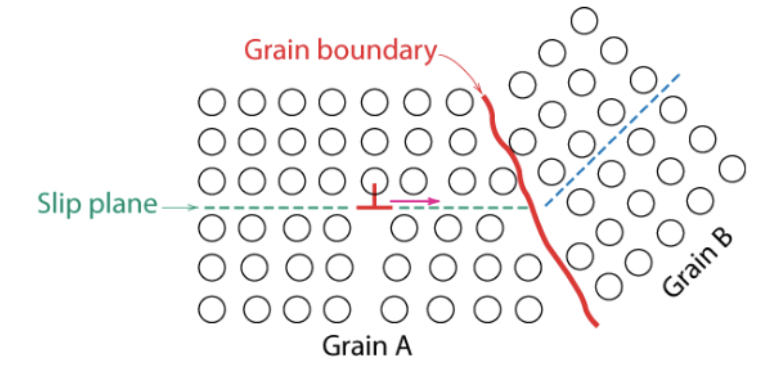
\includegraphics[width=0.5\linewidth]{./figures/f8_5.png}
  \label{fig:f8_5}
\end{figure}

If ones grains are not too coarse or too fine one can approximate the yield strength of a material using the \textit{Hall-Petch equation}.
\[ 
\sigma_y = \sigma_0 + \frac{k_y}{\sqrt{d}}
\]
where the constant $k$ and the ``original'' yield strength $\sigma_0$ are material-dependent constants and $d$ is the average grain diameter.


\subsection{Solid-solution strengthening} \label{sec:sss}
A solid solution occurs when one or more types of solute atoms (impurity atoms) dissolve into a host lattice (the solvent) without forming a separate phase. These solute atoms either occupy the substitutional or interstitial spots in the lattice (see \autoref{sec:interstitial} and \autoref{sec:substitutional}). Substitutional atoms that are smaller than the atoms in the host lattice produce tensile strain and vice versa. Interstitial atoms (like carbon in iron) produce significant lattice distortions because they sit in the spaces between host atoms, pushing them apart and generally creating compressive strain fields around themselves.

\begin{figure} [ht]
  \centering
  \caption{Tensile and compressive strains around an edge dislocation}
  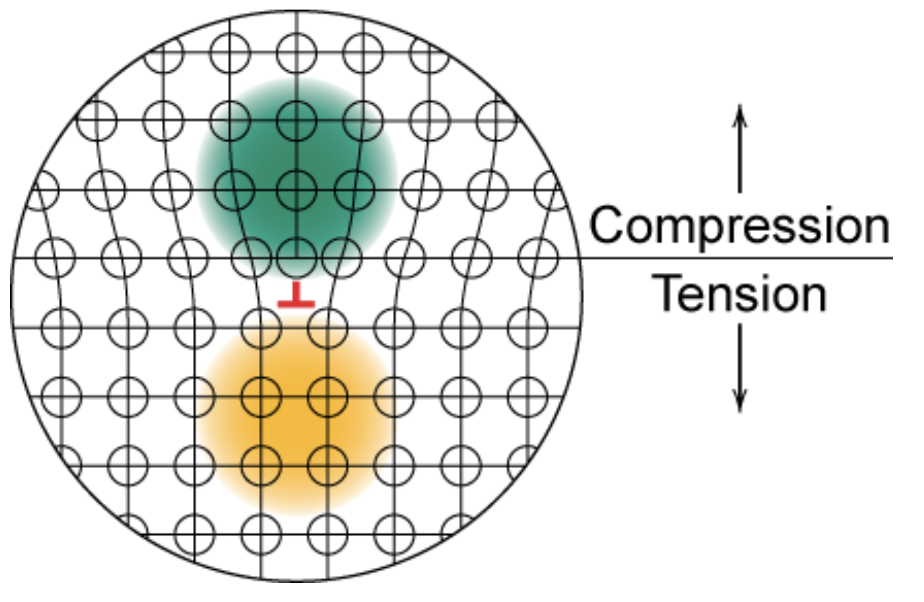
\includegraphics[width=0.5\linewidth]{./figures/f8_6.png}
  \label{fig:f8_6}
\end{figure}

Around dislocations the lattice structure is strained. On \textbf{\autoref{fig:f8_6}} is an illustration of the tensile and compressive strains around an edge dislocation. Dislocations carry around these strain fields. If a solute atom also introduces a strain in the lattice, the interaction between the solute atom’s strain field and the dislocation’s strain field can either:
\begin{itemize}
  \item Reduce the overall strain energy if they have opposite “signs” (e.g., a solute that produces tensile strain is attracted to a region of compressive strain around the dislocation).
  \item Increase the strain energy if they have the same sign (e.g., both produce compressive strain).
\end{itemize}
But because nature tends to minimize energy, a solute atom will be attracted to the region of the lattice around a dislocation that best accommodates (i.e., partially cancels) its own strain. In this way, the solute atoms sort of ``pin'' the dislocations because they want to maintain the minimized strain energy -- if the dislocations start moving the solute atoms will also want to move but moving a solute atom is much harder than moving a dislocation.

In general, introducing more solute atoms (up to a solubility limit) increases the strength and hardness of the metal even more. A mathematical empirical relationship for the yield stress in a solid solution is
\[ 
\sigma_y = \sigma_0 + k C^{n}
\]
where $\sigma_0$ is the yield strength of the pure metal, $C$ is the solute concentration, and $k$ and $n$ are constants that depend on the specific alloy system. It should be stressed that the above expression only is empirical and it should mostly be used to get an idea of how the effect changes with changing amounts of solute. 

\subsection{Strain hardening (Cold working)}
Strain hardening is the process of plastically deforming a metal at a temperature below the metals recrystallization temperature (you often just use room-temperature for most metals), which in turn makes the metal stronger. This deformation often reduces the cross-sectional area of the metal (e.g. a metal sheet will become thinner when rolled).

As you deform a metal you will increase the dislocation density as new dislocations are formed and already existing dislocations multiply (can go from $10^6$ - $10^8$ $\text{dislocations} / \unit{m^2} $ in an annealed metal to $10^10$ - $10^12$ $\text{dislocations} / \unit{m^2} $ in a metal that has undergone significant cold working). When many dislocations are present at once they will start to interact with each other and entangle. Along the same line of thought as in \textbf{\autoref{sec:sss}} these dislocations will try to organize themselves in a way that minimizes energy. When the dislocations start to entangle they also ``pin'' each other in place as moving through another dislocation or too close to another dislocation introduces significant lattice strain.

The degree of strain hardening is measured in $\% \mathrm{CW}$ (percent cold work) which is a way to quantify the amount of plastic deformation introduced. This is
\[ 
\% \mathrm{CW} = \frac{A_0 - A_d}{A_0} \times 100 \%
\]
where $A_0$ is the original cross section of the metal and $A_d$ is the cross section of the metal after deformation. A higher $\% \mathrm{CW}$ means there is a higher dislocation density and therefore that the metal is stronger.

If one chooses to heat treat a strain hardened metal one changes the structure of the cold worked metal. More precisely, if a strain hardened metal is heated to a temperature above its recrystallization temperature (a process known as annealing) the dislocation density will fall and the metal will become more and more like it was before strain hardening. This is shown in \textbf{\autoref{fig:f8_7}}, where the effect of cold working is almost completely gone in the ``grain growth'' part of the annealing diagram. 

\begin{figure} [ht]
  \centering
  \caption{Effect of annealing on temperature}
  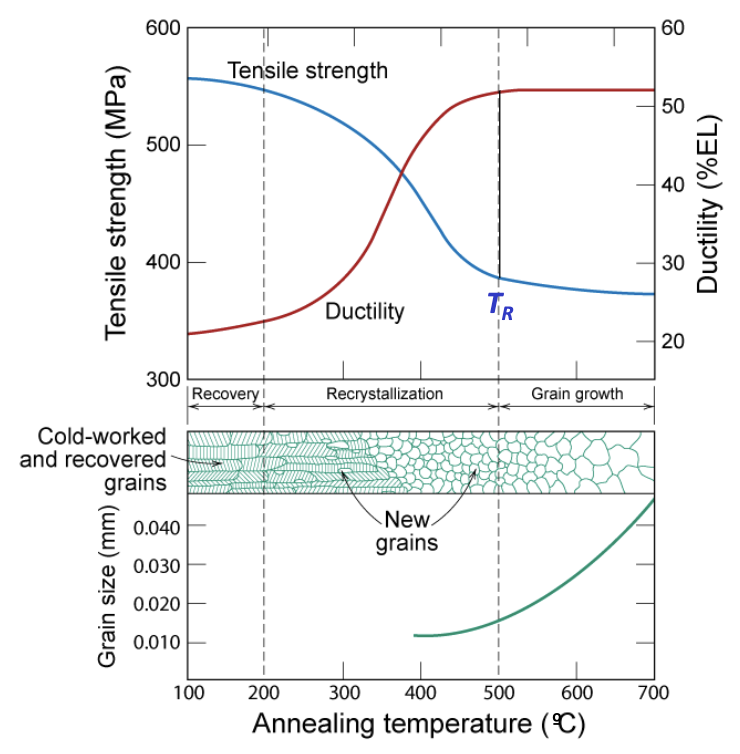
\includegraphics[width=0.45\linewidth]{./figures/f8_7.png}
  \label{fig:f8_7}
\end{figure}
